\lstset {language=C++}
\chapter{Blueprints en C++}

Om de scheiding tussen c++ en Blueprints concreet te maken verdelen wij gameplay logica in de volgende vragen:

\begin{itemize}
	\item Wanneer moet iets gebeuren
	\item Wat moet er gebeuren
	\item Hoe moet dit gebeuren
\end{itemize}

Door deze scheiding wordt het makkelijker om de keuze tussen een c++ en een Blueprint implementatie te maken en kunnen er een aantal richtlijnen opgezet worden.

\section{Wanneer}
De wanneer vragen zijn vaak makkelijk te beantwoorden, bijvoorbeeld als de speler geraakt word door een projectiel wil ik dat geluid x afgespeeld word, maar moeilijk te coderen door hun asynchrone natuur. Een van de krachtigste voordelen van een Visuele programmeer taal is dat de flow van een programma uitgedrukt kan worden door middel van de lijnen tussen nodes. Neem bijvoorbeeld het afspelen van een geluid 1 seconden nadat de speler dood gaat.
C++
We registeren eerst een functie die aangesproken kan worden door de timeout en het geluid wat afgespeeld word in de header

\begin{lstlisting}	
/** Plays a sound x seconds after the death of the player*/
void AfterDeathSoundTimeOut();

/** Sound to play each time we fire */
UPROPERTY(EditAnywhere, BlueprintReadWrite, Category=Gameplay)
class USoundBase* DeathSound;
\end{lstlisting}

Vervolgens word deze functie geïmplementeerd in de .cpp

\begin{lstlisting}
void Adpi_unreal_colosseumCharacter::AfterDeathSoundTimeOut() 
{
	UGameplayStatics::PlaySoundAtLocation(this, FireSound, GetActorLocation());
}
\end{lstlisting}

En word de timeout voor het geluid gezet tijdens het doodgaan van de speler.

\begin{lstlisting}
void Adpi_unreal_colosseumCharacter::OnDeath(const FDeathReason Reason)
{
	// death logic
	...

	FTimerHandle UnusedHandler= FTimerHandle();
	GetWorld()->GetTimerManager().SetTimer(
		UnusedHandler, 
		this, 
		&Adpi_unreal_colosseumCharacter::AfterDeathSoundTimeOut, 
		1.0f
	);
}
\end{lstlisting}

We zijn hier dat de gerelateerde code op drie verschillende plekken komt te staan, tussen niet relevante code in. Pas na het lezen van de code op de drie verschillende plekken word het duidelijk wat de complete functionaliteit is. Er zijn hier natuurlijk hulpmiddel voor zoals opmerkingen boven de code te plaatsen maar bij elke extra taak die, asynchroon, uitgevoerd moet worden word de code complexer en moeilijker te volgen. De lezer moet namelijk alle gerelateerde functionaliteit in zijn geheugen hebben.
Blueprints
In Blueprints zou deze logica er als volgt uit zien:

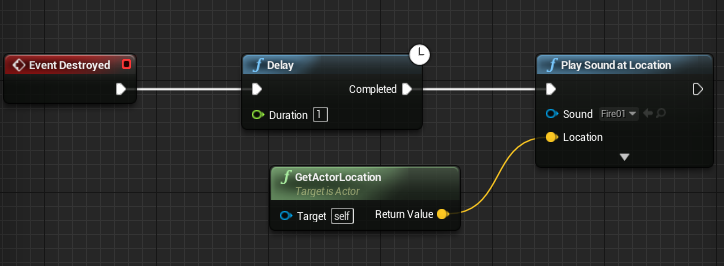
\includegraphics{OnDestroyedSoundDelay}

In de blueprint implementatie is het in een oog opslag duidelijk dat er een geluid afgespeeld word op de locatie van de speler een seconde nadat deze deze dood gaat. De logica bevind zich op de dezelfde plek en de witte lijnen geven de flow van de logica aan. 

Een ander groot verschil dat we hier zien is dat er voor iets simpels als een vertraging in tekstuele code naast de standaard kennis van de c++ syntax ook kennis nodig is van de volgende concepten:

\begin{itemize}
	\item Pointers
	\item Pass by reference
	\item Function references
	\item Namespaces
	\item Out parameters (de UnusedHandler)
	\item Floats
	\item Types
	\item Macros. 
\end{itemize}

Terwijl in Blueprints all deze concepten verborgen zijn in de nodes. Het verbergen van de onderliggende werking van functionaliteit is een thema wat vaker terugkomt in programmeren en wordt aangemoedigd. Het verbergen van deze logica heeft als gevolg dat er zonder programmeer kennis de wanneer logica geïmplementeerd kan worden.

\section{Wat}

Het plaatsen van de wat logica in Blueprints of c++ is lastiger om te bepalen. Voor de logica die de niet-programmeurs schrijven is c++ geen optie en moet dit wel in Blueprints maar voor programmeurs ligt dit iets lastiger. Het probleem ontstaat voornamelijk bij conditionele logica.

Complexe algorithmes zijn altijd makkelijker in C++ voor zowel leesbaarheid als onderhoudbaarheid. Daarnaast is de scheiding van Algoritmes met de rest van de code belangrijk voor 

\section{Hoe}
Met de hoe vraag word de interne werking van een functionaliteit bedoelt waaronder ook de integratie met de rest van het programma, denk aan integratie met de rest van de engine, lifecycles, overerving en performance.

\subsection{Conditionele Logica}

Als we de conditionele logica van het afvuren van de events van een .
LookEventsComponent[zie hoofstuk ?] in c++ en blueprints met elkaar vergelijken.
Bijlage 1: Tick functie van de LookEventsComponent 
Bijlage 2: Conditional logic van Tick functie van LookEvents in Blueprints
Zijn beide varianten moeilijk te lezen. Voor iemand die niet codeert ziet de Blueprints variant er waarschijnlijk begrijpgaarder uit maar de complexiteit komt voornamelijk door de logica zelf en in tekstuele code zijn er een aantal manieren om dit soort constructies kleiner te maken zoals:

\begin{lstlisting}
if (bActive != true || (bShouldUsedOnce && TimesUsed > 0) || bIsInTimeOut == true) 
{
	return;
}
\end{lstlisting}
In vergelijking met 

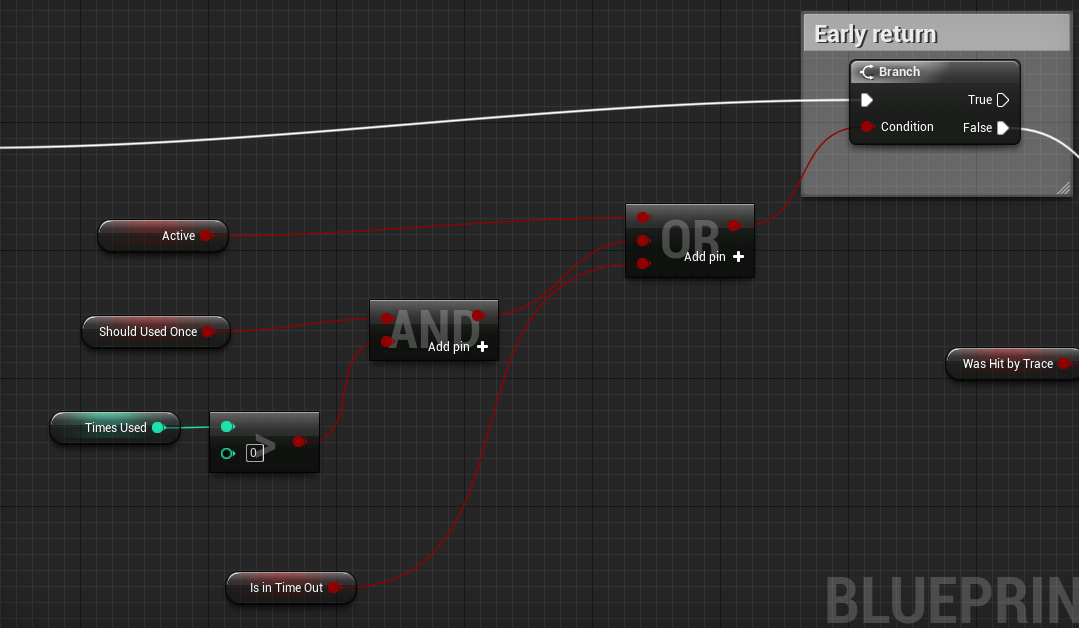
\includegraphics{EarlyReturnBluePrint}

Een ander voorbeeld is de volgende functie die bepaald of de trigger van een LookEventsComponent onderdeel was van een trace.

\begin{lstlisting}
FHitResult ULookEventsComponent::WasHitByTrace(const TArray<FHitResult> HitResults) 
{
	UObject* Trigger = (bIsBeingWatched) ? UnSeenTrigger : SeenTrigger;

	for (auto& HitResult : HitResults)
	{
		UObject* HitObject = (Trigger->IsA(AActor::StaticClass())) ? Cast<UObject>(HitResult.GetActor()) : Cast<UObject>(HitResult.GetComponent());	

		if (HitObject == Trigger)
		{
			if (bShouldDrawTriggerDebug) {
				DebugTrigger(HitObject, 0.1f);
			}
			return HitResult;
		}
	}
	return FHitResult();
}
\end{lstlisting}

In vergelijking met:

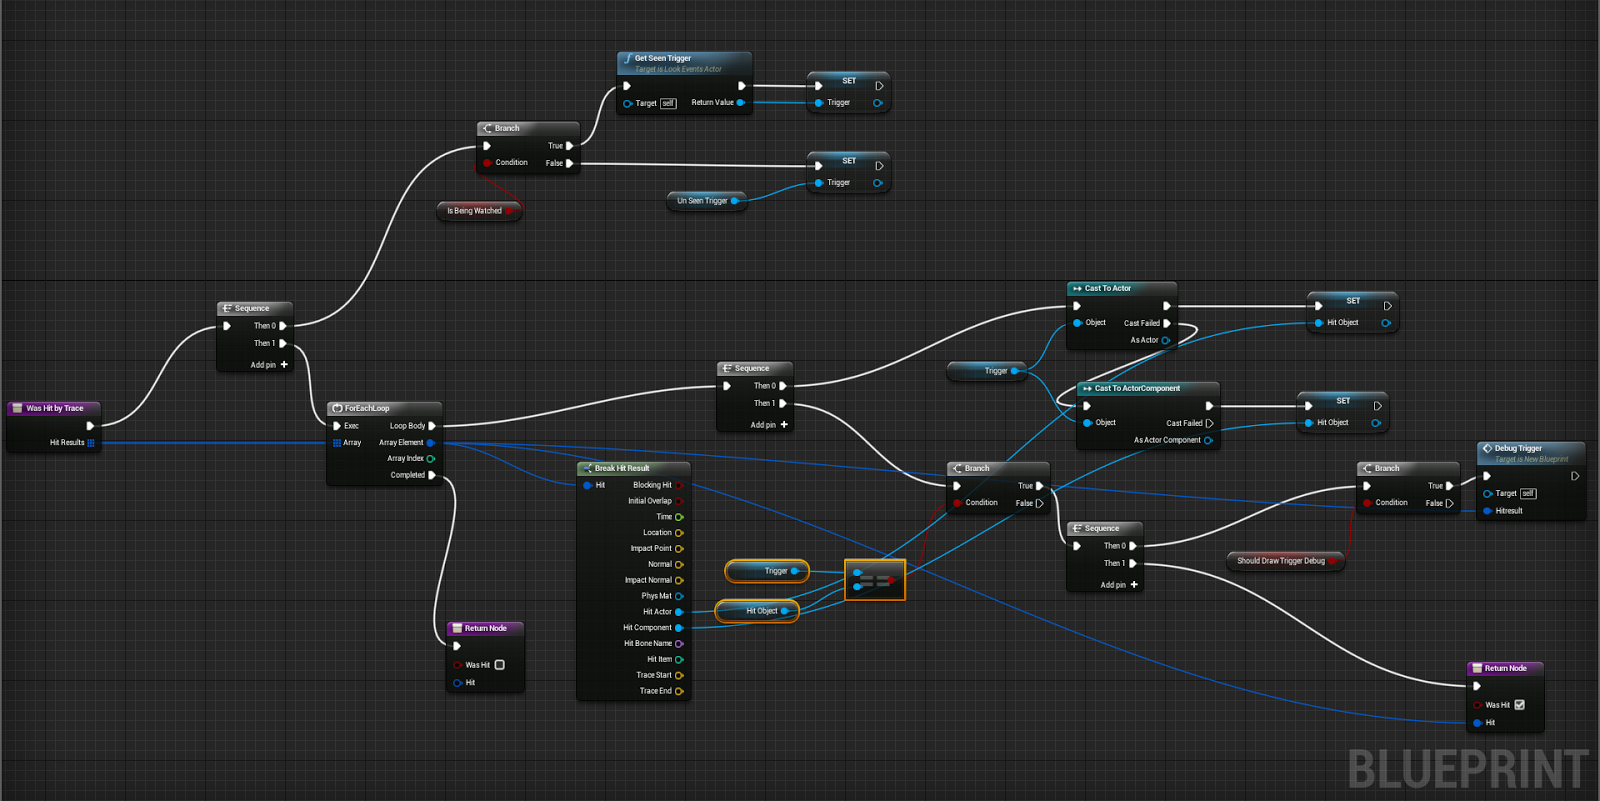
\includegraphics{WasHitBytTraceBluePrintExample}

Voor complexe conditionele logica is c++ sneller te begrijpen en geeft meer mogelijkheden om dit te versimpelen. 

\section{Debugging}
Naast een kleine verbetering in leesbaarheid heeft het schrijven van logica in c++ een ander belangrijke voordelen. Namelijk de voordelen van een code editor. Dit geeft namelijk uitgebreide debug, zoek en meta informatie. 

De error’s die de Unreal Engine 4 voor je genereed zijn niet altijd even duidelijk, voornamelijk error’s die pas tijdens het packagen van een project ontstaan, en het vinden van een foutieve blueprint kan extreem lastig zijn. Bijna elk element in de Unreal Engine 4 kan blueprint code bevatten. En elk element op zich kan die blueprints weer in kleinere elementen verdelen. Deze elementen bevinden zich tussen alle andere soorten assets zoals Meshes, Animaties, Deciscion Trees, Materials, Textures etc en het zoeken van een onbekende fout hierin is extreem lastig.

Als de foutieve code in c++ had gestaan kan er altijd door middel van een stack trace gekeken worden in welke functie het fout gaat en kan er gezien worden welke functie die functie aansprak en verder omhoog. 

Het auto aan vullen van functie namen en informatie tonen over functies door middel van de JavaDoc opmerking notatie versimpelt het schrijven van complexe code die gebruikt maakt van de Unreal Engine 4. 

\section{Performance}
Een ander belangrijk onderdeel van de hoe logica is performance. De performance van Blueprints is namelijk lager dan dat van c++. In de hoe en wat vraag is dit verschil compleet onmerkbaar maar in code wat vaak, bijvoorbeeld in de loop van een game, word uitgevoerd kan het verschil merkbaar worden.
In c++ is er ook veel meer controle over de manier waarop de computer de logica je kan aan de code ook zien hoe de computer dit interpreteer, in Blueprints is dit een stuk minder duidelijk. Dit zorgt ervoor dat op een lager niveau optimalisaties mogelijk zijn. 

Daarnaast is het makkelijker om complexe optimalisaties te schrijven op een onderhoudbaare manier. Als er bijvoorbeeld een performance probleem ontstaat in het aantal raytraces wat de LookEventsComponents nodig hebben is het mogelijk om een cache te schrijven voor de ray traces waar de LookEventsComponent een trace uit vraagt als deze trace dan al eerder door een andere LookEventsComponent berekend is krijg hij de resultaten van die trace inplaats van een nieuwe trace te maken.

De mogelijkheid van dit soort optimalisaties, de debugging mogelijkheden en de leesbaarheid van complexe logica 

Workflow
Git
c++